\documentclass[12pt]{article}
\usepackage[left=3cm,right=3cm,top=2cm,bottom=2cm]{geometry} % page
                                                             % settings
\usepackage{amsmath} % provides many mathematical environments & tools
\usepackage[spanish]{babel}
\usepackage[doument]{ragged2e}

% Images
\usepackage{graphicx}
\usepackage{float}

% Code
\usepackage{listings}
\usepackage{xcolor}
\definecolor{gray}{rgb}{0.5,0.5,0.5}
\newcommand{\n}[1]{{\color{gray}#1}}
\lstset{numbers=left,numberstyle=\small\color{gray}}

\selectlanguage{spanish}
\usepackage[utf8]{inputenc}
\setlength{\parindent}{0mm}

\usepackage{enumerate}

\begin{document}

\title{Timbálico: Grafo PHIGS}
\author{David Cabezas}
\date{\today}
\maketitle

He creado un modelo jerárquico con múltiples componentes que se mueven
de diversas formas, lo he bautizado como Timbálico. Consta de un
soporte con dos brazos, cada uno con una hélice que se desplaza por él
a la vez que gira y una pelota en el extremo que se infla y desinfla.

\subsection*{Grafo PHIGS}
\vspace{-5mm}

\begin{figure}[H]
 \hspace{-30mm} 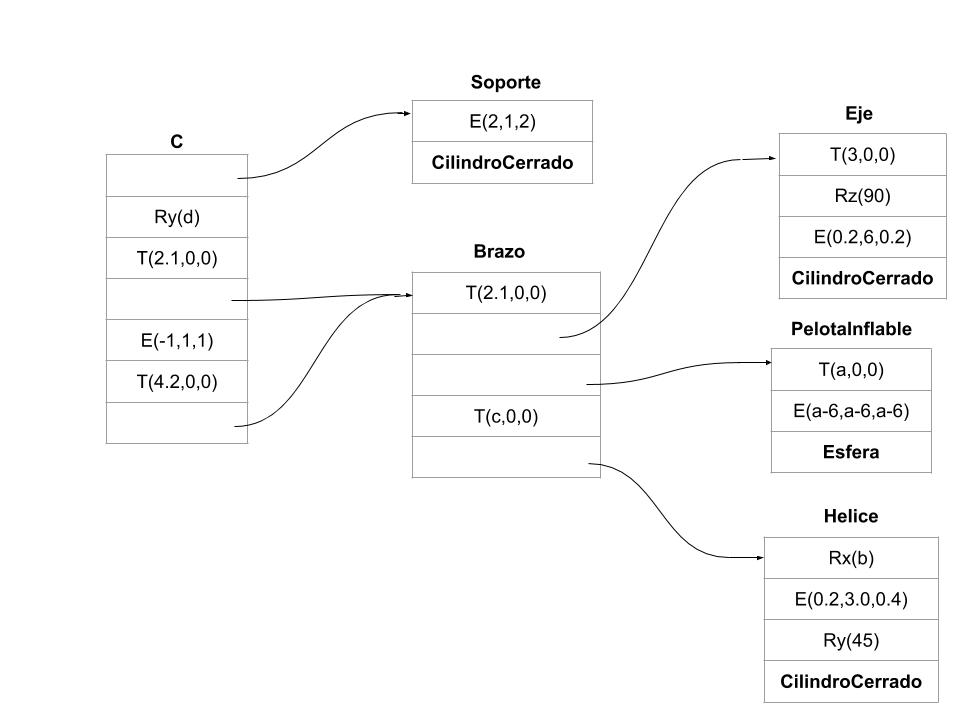
\includegraphics[width=200mm]{PHIGS-timbalico}
\end{figure}

\subsection*{Parámetros / Grados de libertad}

El Timbálico tiene 7 grados de libertad, que detallo a continuación:
\begin{enumerate}
\item \textbf{Rotación del Timbálico:}
  Los brazos del Timbálico rotan sobre el eje $Y$, alrededor del soporte. \\ $d=90t_{sec}$
\item \textbf{Rotación y traslación de la PelotaInflable 1:}
  La PelotaInflable 1 se agranda y empequeñece, su radio oscila entre 1 y 2 y su centro se desplaza para que su superficie siempre quede en el extremo del Eje del Brazo 1. \\ $a=7.5+0.5\sin(t_{sec}\pi/2)$
\item \textbf{Rotación y traslación de la PelotaInflable 2:}
  La PelotaInflable 2 se agranda y empequeñece, su radio oscila entre 1 y 2 y su centro se desplaza para que su superficie siempre quede en el extremo del Eje del Brazo 2. \\ $a=7.5+0.5\sin(t_{sec}\pi/2)$
\item \textbf{Rotación de la Helice 1:}
  La Helice 1 rota sobre el Eje del Brazo 1 (inicialmente el eje $X$).
  \\ $b=360t_{sec}$
\item \textbf{Rotación de la Helice 2:}
  La Helice 2 rota sobre el Eje del Brazo 2 (inicialmente el eje $X$).
  \\ $b=360t_{sec}$
\item \textbf{Traslación de la Helice 1:} La Helice 1 recorre el Eje
  del Brazo 1 (inicialmente el eje $X$), oscilando entre el Soporte y
  la PelotaInflable1. \\ $c=2.95+2.95\sin(t_{sec}\pi/4)$
\item \textbf{Traslación de la Helice 2:} La Helice 2 recorre el Eje
  del Brazo 2 (inicialmente el eje $X$), oscilando entre el Soporte y
  la PelotaInflable1. \\ $c=2.95+2.95\sin(t_{sec}\pi/4)$
\end{enumerate}

\subsection*{Nodos terminales}

Sólo he necesitado dos tipos de mallas indexadas para los nodos terminales. \\

Una es la Esfera de revolución que hice en la práctica 2, la he pintado de rojo. \\

El otro es CilindroCerrado, una modificación del cilindro de
revolución, le he puesto tapas y lo he centrado en el origen (las
bases están a las alturas $y=-0.5$ e $y=0.5$). Lo he transformado para
el soporte (pintado de marrón) y para los ejes (pintado de azul).

\end{document}
